\documentclass[11pt]{article}

\usepackage[T1]{fontenc}
\usepackage[expert]{lucidabr}
\usepackage{graphicx}
\usepackage{enumitem}
\setlist{itemsep=0.2ex,parsep=0.2ex}
\usepackage[usenames]{color}
\usepackage{epstopdf}
\usepackage{amsmath}
\usepackage[margin=5pt,font=footnotesize,labelfont=bf,textfont=md,format=hang,indention=-1cm,justification=raggedright]{caption}
\usepackage{wrapfig}

\newcommand{\kc}{\textsf{kCARTA}\xspace}
\newcommand{\sa}{\textsf{SARTA}\xspace}
\newcommand{\sasc}{\textsf{SARTA-CLOUDY}\xspace}
\newcommand{\pcrtm}{\textsf{PCRTM}\xspace}

% figure1 figure1-caption figure1-label figure2 figure2-caption figure2-label
\newcommand{\dfigure}[6]
{
\begin{figure}
  \begin{minipage}[t]{0.47\textwidth}
  \centering
  \includegraphics[width = 1.00\textwidth]{#1}
   \caption{#2}  \label{#3}
  \end{minipage}
  \hfil
  \begin{minipage}[t]{0.47\linewidth}
  \centering
  \includegraphics[width = 1.00\textwidth]{#4}
   \caption{#5}  \label{#6}
  \end{minipage}
\end{figure}
}

\usepackage{xspace}
\newcommand{\wn}{cm$^{-1}$\xspace}
\newcommand{\um}{$\mu m$\xspace}
\newcommand{\cd}{CO$_2$\xspace}
\newcommand{\water}{H$_2$O\xspace}
\newcommand{\methane}{CH$_4$\xspace}
\newcommand{\nitrogen}{N$_2$\xspace}
\newcommand{\nitrous}{N$_2$O\xspace}
\newcommand{\oxygen}{O$_2$\xspace}
\newcommand{\ozone}{O$_3$\xspace}
\newcommand{\mydeg}{\mbox{$^\circ$}}

%---------------------------------------------------------------------------
\makeatletter
\renewcommand{\section}{\@startsection {section}{1}{\z@}%
                                   {-3.5ex \@plus -1ex \@minus -.2ex}%
                                   {2.3ex \@plus.2ex}%
                                   {\reset@font\large\bfseries}}
\renewcommand{\subsection}{\@startsection{subsection}{2}{\z@}%
                                     {-3.25ex\@plus -1ex \@minus -.2ex}%
                                     {1.5ex \@plus .2ex}%
                                     {\reset@font\normalsize\bfseries}}
\makeatother
%---------------------------------------------------------------------------
% Indent captions a little
%\setlength{\captionmargin}{10pt}
\parindent=1.2em
\parskip=0.5ex

%  For the tables
\def\tstrut{\vrule height 2.5ex depth 1.2ex width 0pt}
\def\tstruta{\vrule height 0ex depth 1.2ex width 0pt}
%---------------------------------------------------------------------------
% If use fancyhdr
% \lhead{}
% \rhead{}
% \chead{}
% \lfoot{\small\sf Page \thepage\ of \pageref{LastPage}}
% \rfoot{\small\sf L. Strow/UMBC}
% \cfoot{\small\sf AIRS and IASI Intercal}
%\renewcommand{\headrulewidth}{0pt}  % only with fancyhdr
%\pagestyle{plain}
\usepackage{geometry}
\geometry{letterpaper,margin=1.0in,vcentering}

\title{\textsf{SARTA CLOUDY}: A Fast Forward Model Version of
  \textsf{SARTA}\\ with Cloud/Aerosol Scattering}

\author{S. De Souza-Machado, L. L. Strow, S. E. Hannon \\
      University of Maryland Baltimore County, Baltimore, MD 21250 USA}

    \begin{document}

    \maketitle

    \begin{abstract}

      The \textsf{SARTA CLOUDY} code is a modification of UMBC's \sa
      clear-sky fast radiative transfer algorithm, allowing users to
      compute synthetic infrared radiances for the AIRS instrument, in
      the presence of clouds and aerosols. By re-parameterizing the
      cloud scattering parameters into effective optical depths, the
      effect of clouds on upwelling radiation from the Earth's
      atmosphere is effectively recast as that of (an) additional
      absorbing gas(es), which allows us to use the efficient
      radiative transfer algorithm of the clear sky code. The liens of
      the code are that model vertical cloud fields (from eg ECMWF)
      need to be reshaped into at most two slab clouds. However,
      comparisons against packages which uses sophisticated algorithms
      (eg maximal overlap clouds and scattering trained on DISORT
      algorithm) shows that the \textsf{SARTA CLOUDY} code produces
      radiances accurate to about 3K (converted to equivalent
      Brightness Temperature)

    \end{abstract}

    \section{Introduction}

    This document gives an overview of \sasc, a version of UMBC's
    clear-sky \sa algorithm that includes scattering by clouds an
    aerosols.  Our goal was to produce a relatively accurate code, but
    with an emphasis on speed, in order to allow it for use in a
    production cloudy scene retrieval system.  \sasc code is very
    similar to code in our \sa clear-sky algorithm, making it
    relatively easy to use as a replacement for users of \sa.  The
    code is based on an approach that models the effects of cloud and
    aerosols as additional absorptive gases, so that the radiative
    transfer retains its speed and efficiency.  In addition, \sasc
    also includes scattering by in-coming solar radiation in the
    shortwave, albeit with somewhat lower accuracy than the scattering
    in the longwave.  However, slight in-accuracies in scattering
    \emph{may} be relatively un-important in a retrieval system where
    one can only solve for a few cloud parameters since a more
    accurate algorithm will most likely be using cloud microphysical
    parameters and cloud structures that have significant errors
    relative to the observations.

    We begin by outlining the clear sky monochromatic algorithm,
    followed by a discussion of the scattering model we chose to use
    for the monochromatic case. We then follow with a brief discussion
    of the challenges in making a code for polychromatic clear sky
    transfer, and how the scattering algorithm can be easily adapted
    to work in this polychromatic case as well.

    We have already successfully used \sasc to retrieve dust optical
    depths and heights for individual AIRS Fields-of-Views
    \cite{mac:10}.  For a fixed dust layer height, and a handful of
    AIRS channels, three iterations for convergence were done in
    several milliseconds, for each AIRS pixel. We also summarize how
    we convert Numerical Weather Prediction Model (NWP) fields into
    clouds fields that can be processed inside of \sasc and show some
    comparisons of window channel radiances computed using ECMWF/ERA
    fields versus actual AIRS observations.

    We also show limited comparisons between radiances produced by
    \sasc versus those produced by a more sophisticated algorithm.
    These comparisons are complicated by issues related to how the
    algorithm handles NWP cloud overlap, which is not directly
    applicable to the use of these algorithms for remote sensing
    retrievals.

    \section{Monochromatic Clear sky Radiative transfer algorithm}

    As a monochromatic beam of radiation propagates through a layer,
    the change in diffuse beam intensity $R(\nu)$ in a plane parallel
    medium is given by the standard Schwartschild equation
    \cite{lio:80,goo:89,edw:92}
    \begin{equation}
      \mu \frac{dR(\nu)}{dk_{e}} = -R(\nu) + J(\nu)
      \label{eqn:sch}
    \end{equation}
    where $\mu$ is the cosine of the viewing angle, $k_{e}$ is the
    extinction optical depth, $\nu$ is the wavenumber and $J(\nu)$ is
    the source function. For a nonscattering ``clear sky'', the source
    function is usually the Planck emission $B(\nu,T)$ at the layer
    temperature $T$, leading to an equation that can easily be solved
    for an individual layer. Dividing the atmosphere into layers and
    propagating the solution through the layers, the final upwelling
    radiance (for a downlooking instrument) can be written in terms of
    four components :

\begin{equation}
  R(\nu) = R_{s}(\nu) + R_{\text{layer emission}}(\nu) + R_{\text{th}}(\nu) + R_{\text{solar}}(\nu)
  \label{eqn:sch_detail}
\end{equation}
which are the surface, layer emissions, downward thermal and solar
terms respectively. The terms in the equation are relatively
straightforward, and the resulting algorithm is usually quite
efficient.

% \begin{wrapfigure}{l}{0.45\textwidth}
%   \centering
%   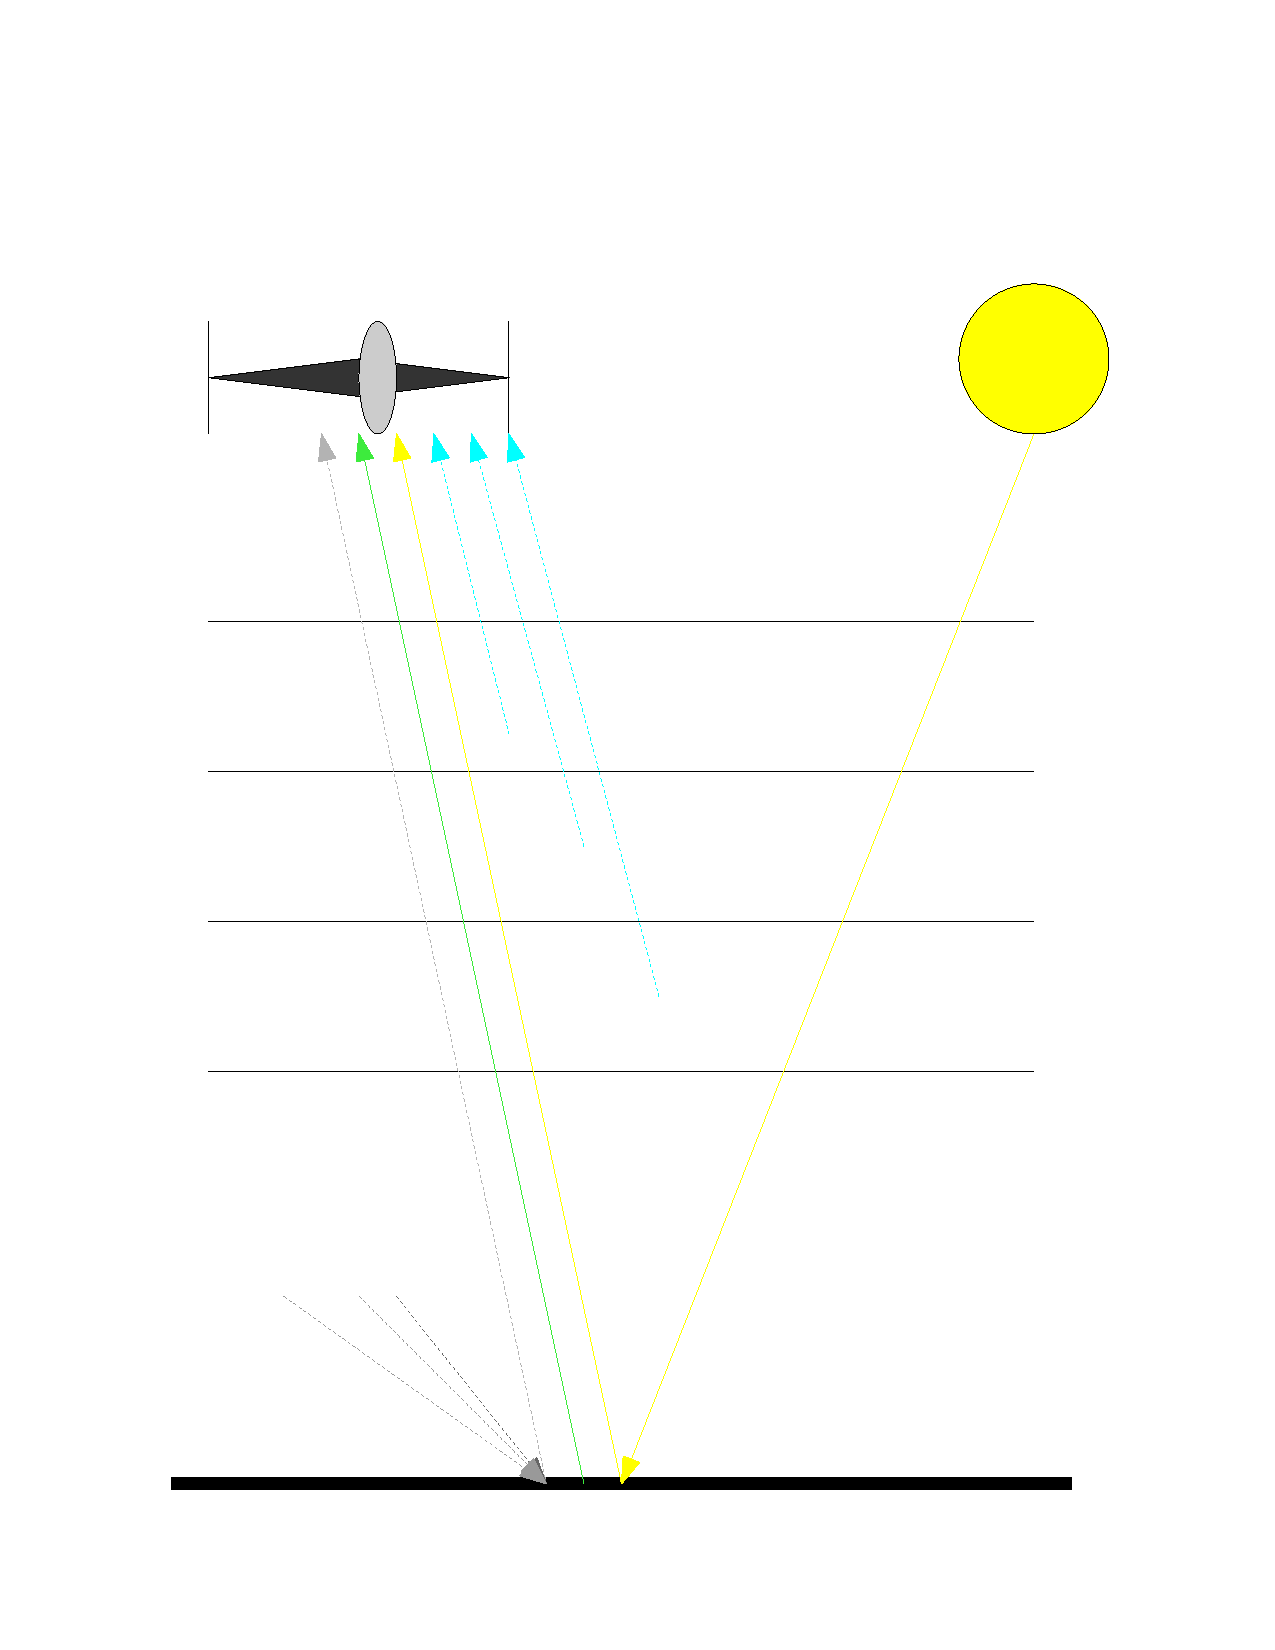
\includegraphics[width=0.45\textwidth]{Figs/radiation1.pdf}
%   \caption{Illustration of contributions to measured Top Of
%   Atmosphere radiance : (blue) layer emission, (green) surface,
%   (yellow) solar and (gray) background thermal}
% \end{wrapfigure}
Our monochromatic code \kc indexes the atmosphere so that layer $1$ is
the bottom and $N$ (=100) the uppermost. Denoting $B(T)$ as the Planck
function, $T_{s}$ as the skin surface temperature, $\epsilon_{s}$ as
the surface emissivity, $\theta$ as the satellite viewing angle,
$\theta_{\text{solar}}$ as the sun zenith angle, $\tau_{i}(\nu)$ as
the transmission of layer $j$ ($\tau_{i}(\nu) = \exp^{-k_{i}(\nu)}$),
$\tau_{j \rightarrow m}(\nu)$ as the transmission from layer $i$ to
layer $m$, the individual terms are computed in monochromatic codes,
such as \kc as follows.

\subsection{Surface emission}

This is simply the emission from the surface (temperature $T_{s}$),
multiplied by the surface emissivity $\epsilon_{s}$ to account for the
surface not being a perfect black body, and attenuated by absorption
due to the atmosphere.
\begin{eqnarray*}
  R_{s}(\nu) & = & \epsilon_{s} B(\nu,T_{s}) \tau_{1 \rightarrow N}(\nu,\theta)
\end{eqnarray*}

\subsection{Layer emission}

As the radiation emitted from the surface propagates up, it is
absorbed by the layer of gas above it, and then re-emitted. This
atmospheric emission happens layer by layer :
\begin{eqnarray*}
  R_{\text{layer emission}}(\nu) & = & \sum_{i=1}^{i=N} B(\nu,T_{i})
  (1.0 - \tau_{i}(\nu)) \tau_{i+1 \rightarrow N}(\nu,\theta))
\end{eqnarray*}
Layers with negligible absorption ($\tau_{i} \rightarrow 1$)
contribute negligibly to the overall radiance, while those with large
optical depths ($\tau_{i} \rightarrow 0$) ``black'' out radiation from
below.  $(1.0 - \tau_{i}(\nu))$ is the emissivity of the layer while
$(1.0 - \tau_{i}(\nu)) \tau_{i+1 \rightarrow N}(\nu,\theta))$ is the
weighting function $W_{i}$ of the layer.

\subsection{Background thermal radiation}

The atmosphere also emits radiation downward in a manner analogous to
the upward layer emission just discussed. Upon reaching the surface,
this radiance may be reflected upward. At the surface, the magnitude
of this background term is :
\begin{eqnarray}
  R_{\text{th}}^{\text{surface}}(\nu) & = & \sum_{i=N}^{i=1}
  \int_{0}^{2\pi}d\phi
  \int_{0}^{\pi/2} d(\cos\theta) \cos\theta \rho(\theta,\phi)
  \times B(\nu,T_{i}) \times \Delta \tau
  \label{bckgnd_eqn}
\end{eqnarray}
Here $ \Delta \tau = (\tau_{i-1 \rightarrow
  \text{ground}}(\nu,\theta)- \tau_{i \rightarrow
  \text{ground}}(\nu,\theta))$.  Note the summation has been reversed,
as we start out from the top of the atmosphere $N$, and come down to
ground $i=1$.  This background thermal term also depends on the
surface reflectivity $\rho$.  If one assumes that the reflectivity of
the surface is Lambertian, then $\rho$ can be rewritten as $\frac{1 -
  \epsilon_{s}}{\pi}$. This entire background reflected term is
negligible in regions with either strong atmospheric absorption (or no
atmospheric absorption), but in nominal window regions can contribute
as much as 0.5 K of the total radiance when reflected back up to the
top of the atmosphere.

Equation \ref{bckgnd_eqn} involves an angular integration that needs
to be done quickly but accurately. Layer by layer, the Mean Value
Theorem states Eq. \ref{bckgnd_eqn} can be rewritten in terms of an
effective diffusive angle $\theta^{i}_{d}$ at each layer $i$ :
\begin{eqnarray*}
  R_{\text{th}}^{\text{surface}}(\nu) & =
  & \frac{1 - \epsilon_{s}}{\pi} \frac{1}{2} \sum_{i=N}^{i=1}
  B(T_{i}) \left[ \tau_{i-1 \rightarrow \text{ground}}
    (\nu,\theta^{i}_{d1})-\tau_{i \rightarrow \text{ground}}(\nu,\theta^{i}_{d2}) \right]
\end{eqnarray*}
where based on the layer to ground transmissions of the $i,i-1$ $th$
layers, $\theta^{i}_{d1},\theta^{i}_{d2}$ are the optimum diffusion
angles.

The value of $\theta^{i}_{d}$ that is often used is the $\arccos(3/5)$
\cite{lio:80}, especially for low optical depths ($k \le 1$).  A check
of the accuracy of using this angle at all layers against an accurate
computation using Eq. \ref{bckgnd_eqn}, showed that the errors in the
window regions could be larger than 0.2 K, and would be even larger
over land surfaces where the land surface emissivity is as low as
0.8. Instruments such as AIRS have channel radiance accuracies better
than 0.2K, making it important to compute the background thermal
correctly throughout the wavenumber region encompassed by the
spectroscopic \kc database.

As Eq. \ref{bckgnd_eqn} is computationally intensive, we devised the
following.  In an optically deep region, the surface is blacked out
and one need not accurately compute the reflected term, and so
$\arccos(3/5)$ can be used at all layers.

Conversely in an ``optically thin'' region, the layers closest to the
ground contribute most to $R_{\text{th}}(\nu)$ (see discussion of
weighting function above).  For each 25 \wn region, the layer $L$
above which $\arccos(3/5)$ can be safely used, was determined. Below
this layer, we use a lookup table where $\theta^{i}_{d}$ angle is
parameterized as a function of layer-to-ground optical depth (and
hence transmittance).

With surface emissivity set at 0.8, $L$ was chosen such that the
brightness temperature errors at the top of the atmosphere were less
than 0.1K for the sampling of profiles tested. The accuracy was
checked by propagating the thermal background between the top of the
atmosphere and the ground using this method, and comparing it to the
results from using Eq. \ref{bckgnd_eqn}.

\subsection{Solar radiation}

Letting the solar reflectance be denoted by $\rho(\nu)$, then
\begin{eqnarray*}
  R_{\text{solar}}(\nu) & = & \rho(\nu) B_{\text{solar}}(\nu) \cos(\theta_{\text{solar}}) \times \\
  & &                 \tau_{N \rightarrow \text{ground}}(\nu,\theta_{\text{solar}}))
  \tau_{\text{ground} \rightarrow N}(\nu,\theta))
  \Omega_{\text{solar}}
\end{eqnarray*}
$\rho$ is usually (inaccurately) modeled as $\rho = \frac{1 -
  \epsilon_{s}}{\pi}$.  $\Omega_{\text{solar}} =
\pi(r_{s}/d_{se})^{2}$ is the solid angle subtended at the earth by
the sun, where $r_{e}$ is the radius of the sun and $d_{se}$ is the
earth-sun distance. The solar radiation incident at the TOA
$B_{\text{solar}}(\nu)$ comes from datafiles, and is modulated by the
angle the sun makes with the vertical, $\cos(\theta_{\text{solar}})$.

\subsection{\textsf{Monochromatic PCLSAM} scattering algorithm}

\kc can be interfaced with advanced scattering codes such as DISORT
\cite{stam:88} and RTPSEC \cite{dee:98}. While well tested and
numerically very accurate, these codes are complicated, leading to run
times that far longer than for the clear sky case.
% Sergio; I know what you want to say, I think, but too confusing?  In
% addition, the separation of radiative effects into solar and
% terrestrial means, for typical infrared instruments such as AIRS,
% IASI and CRiS, means one can optimize codes to work on either the
% thermal and/or the short wave infrared regions.

We chose to implement a radiative transfer algorithm optimized to work
where scattering is less important than absorption effects. In the
thermal infrared, the effects of scattering due to aerosols and clouds
are small compared to the scatterer absorption, making the
\textsf{PCLSAM} (Parameterization of Cloud Longwave Scattering for use
in Atmospheric Models) scheme \cite{cho:99} very attractive. This
model assumes the downward intensity through a cloud layer is the same
as the Planck emission at the cloud temperature and thus simplifies
the problem, although it typically slightly overestimates the final
TOA radiance. This algorithm changes the optical depth from $k$ to a
parameterized number $k\prime$ as described briefly below; more
details can be found in \cite{cho:99,mat:05}.

For each layer $i$ that contains scatterers, we replace the optical
depth with the total optical depth $k_{\text{total}}(\nu) =
k_{\text{atm}}^{\text{gases}}(\nu) +
k^{\text{scatterer}}_{\text{extinction}}(\nu)$.  However this is
reparameterized as
\[
k\prime(\nu) = k_{\text{total}}(\nu) \times \{ (1-\omega(\nu)
(1-b(\nu)) \}
\]
where the effective single scattering albedo $\omega$ and backscatter
$b$ are obtained from the scatterer-only case $\omega_{0}$ using
\[
\omega(\nu) = \omega_{0}(\nu)
k^{\text{scatterer}}_{\text{extinction}}(\nu)/k_{\text{total}}(\nu)
\]
\[
b(\nu) = (1 - g(\nu))/2
\]
Note that if there are no scatterers in the layer, $\omega(\nu)
\rightarrow 0$ and we recover the clear sky optical depth.

This same parameterization of the optical depth can be repeated for
all the layers which contain scatterers, allowing the radiative
transfer algorithm to be written in the same form as that for clear
sky radiative transfer, with very little speed penalty. Since the
scattering parameters
$k^{\text{scatterer}}_{\text{extinction}},\omega_{0},g$ are stored in
lookup tables as a function of particle size, it is trivial to obtain
the derivatives with respect to size and particle amount. This method
therefore immediately lends itself to be extended to compute
scattering jacobians as well as fluxes, in a manner exactly analogous
to that for clear sky jacobians and fluxes.

We have attempted to account for solar scattering in the shortwave,
but comparing to DISORT and actual AIRS observations, we state this a
significant lien on the code in this spectral region.  We note that
while computing the direct beam scattered solar contribution, we use
the extinction optical depth $k$ in $ \left[ 1 - e^{-k (\frac{1}{\mu}
    + \frac{1}{\mu_{sun}})} \right]$, rather than the parameterized
optical depth $k \prime$.
% Sergio, any estimate of the scattering accuracy in the SWIR You
% can't tell them we have it, it's not good, w/o any estimate.
Some important points to consider:

\begin{itemize}
\item While absorption spectra due to atmospheric gases has sharp
  spectral structure, the crystal bonding, and smoothing over particle
  size distributions, "blurs" out sharp features, resulting in
  spectrally smooth absorption and scattering parameters.
\item Aerosol particles range in size from 0.1 um (smoke) to 4 um
  (dust) in diameter, which means the thermal infrared is typically
  much more sensitive to dust than to smoke.
\item Even for dust, non-sphericity of these particles is not a very
  big issue in the thermal infrared.  As long as realistic refractive
  indices are used, the results of Mie codes, integrated over
  realistic particle size distributions, should suffice to produce
  scattering parameters that can be relied upon.
\item Similarly, water clouds can be assumed to be spherical,
  typically 20 um in diameter, although this can be treated as a
  variable in the code via (fast) look-up tables.
\item Cirrus clouds can contain many different types of shapes or
  "habits", which typically depend on temperature through the height
  of the cloud. Since the resulting ice crystals can be quite large,
  whose shapes can deviate significantly from spherical, Mie codes
  should not be used to produce scattering parameters for use in
  terrestrial radiative transfer codes.  We use cirrus scattering
  parameters for ice aggregates or hexagonal plates, provided by
  Anthony Baran of the UKMO.
\end{itemize}

\section{SARTA Clear Sky Radiative transfer algorithm}

Keeping the surface and layer emission terms, while ignoring the solar
and background thermal terms, the monochromatic clear sky radiative
transfer algorithm can be written as
\begin{eqnarray*}
  R_{\text{toa}}(\nu) & = & \epsilon_{s} B(\nu,T_{s}) \tau_{1 \rightarrow N}(\nu,\theta) + \\
  &   &  \sum_{i=1}^{i=N} B(\nu,T_{i})
  (1.0 - \tau_{i}(\nu)) \tau_{i+1 \rightarrow N}(\nu,\theta)) \\
  & = & \epsilon_{s} B(\nu,T_{s}) \mathcal{T}(\nu,\theta)^{1 \rightarrow N} + \\
  &   &  \sum_{i=1}^{i=N} B(\nu,T_{i}) \{ \mathcal{T}(\nu,\theta)^{i+1\rightarrow N} - 
  \mathcal{T}(\nu,\theta)^{i \rightarrow N} \}
\end{eqnarray*}
from which the top-of-Atmosphere radiance for an AIRS channel would be
given by
\begin{eqnarray*}
  R_{\text{AIRS}}(j) = \int_{\delta \nu_{j}} R_{\text{toa}}(\nu) \text{SRF}_{j}(\nu) d\nu
\end{eqnarray*}

Notice that in both the surface term and the atmospheric emission
term, we deal with layer to space transmittances, which means we need
to take into consideration what is above each layer during the
iteration of the radiative transfer algorithm. For a monochromatic
code, this is not an issue, as Beer's law applies.

On a 2.3 GHz machine, a \kc run from 605-2830 \wn would take about 90
seconds, as optical depths have to be generated for about 900000
wavenumber points (spanning the above interval at 0.0025 \wn spacing)
for each of the 100 layers. The spectral convolution for all 2378
channels using Matlab would add on an additional $\sim$ 10 seconds to
generate one synthetic AIRS clear sky spectrum with the \kc
line-by-line code.

With AIRS providing about 3 million spectra per day, it would clearly
be next to impossible to use \kc in its current guise, to analyze the
data. A fast Stand Alone Radiative Transfer Model (SARTA) was written,
which takes a fraction of the above time (about 0.1 seconds) to
generate one synthetic spectrum. For each AIRS channel, a simplified
view of how this this code works is as follows. The atmospheric gas
absorption for
% \begin{wrapfigure}{l}{0.45\textwidth}
%   \centering
% %   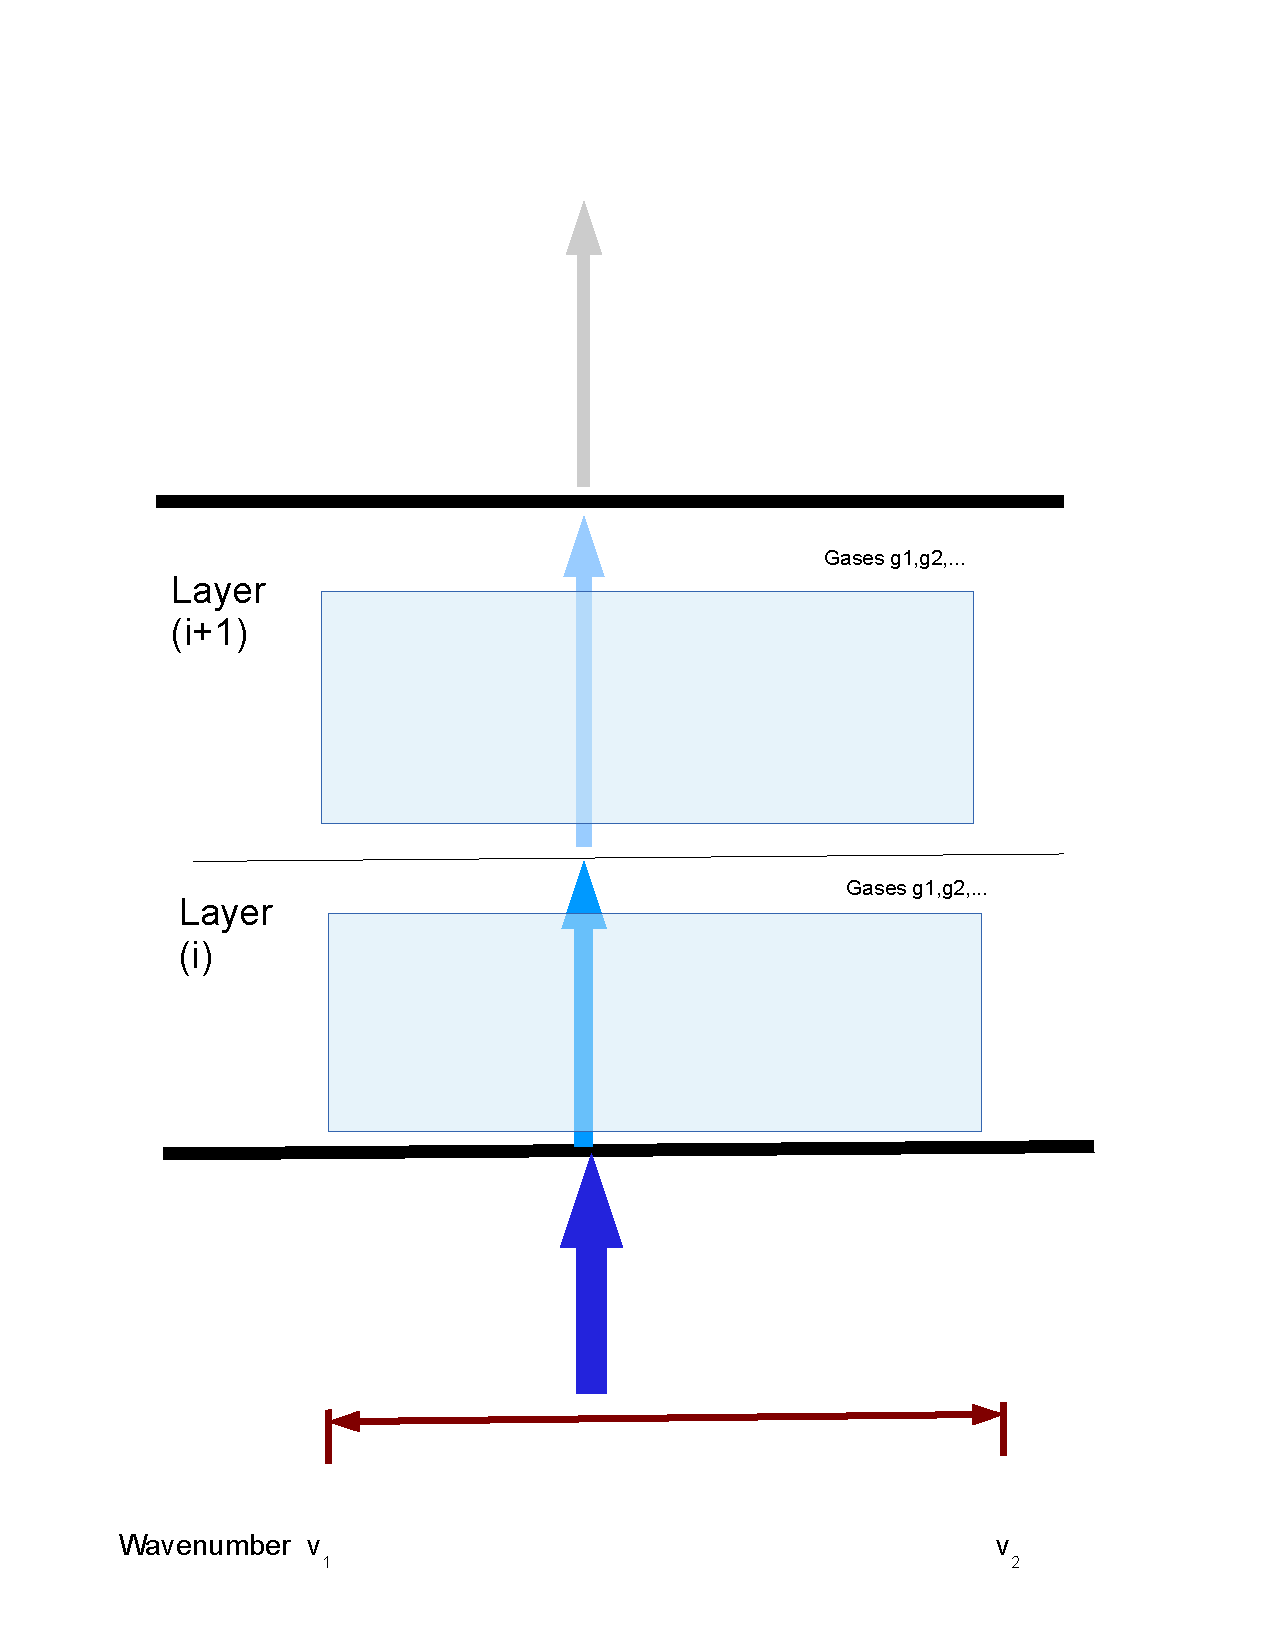
\includegraphics[width=1\textwidth,height=0.5\textheight]{Figs/twolayers.pdf}
%   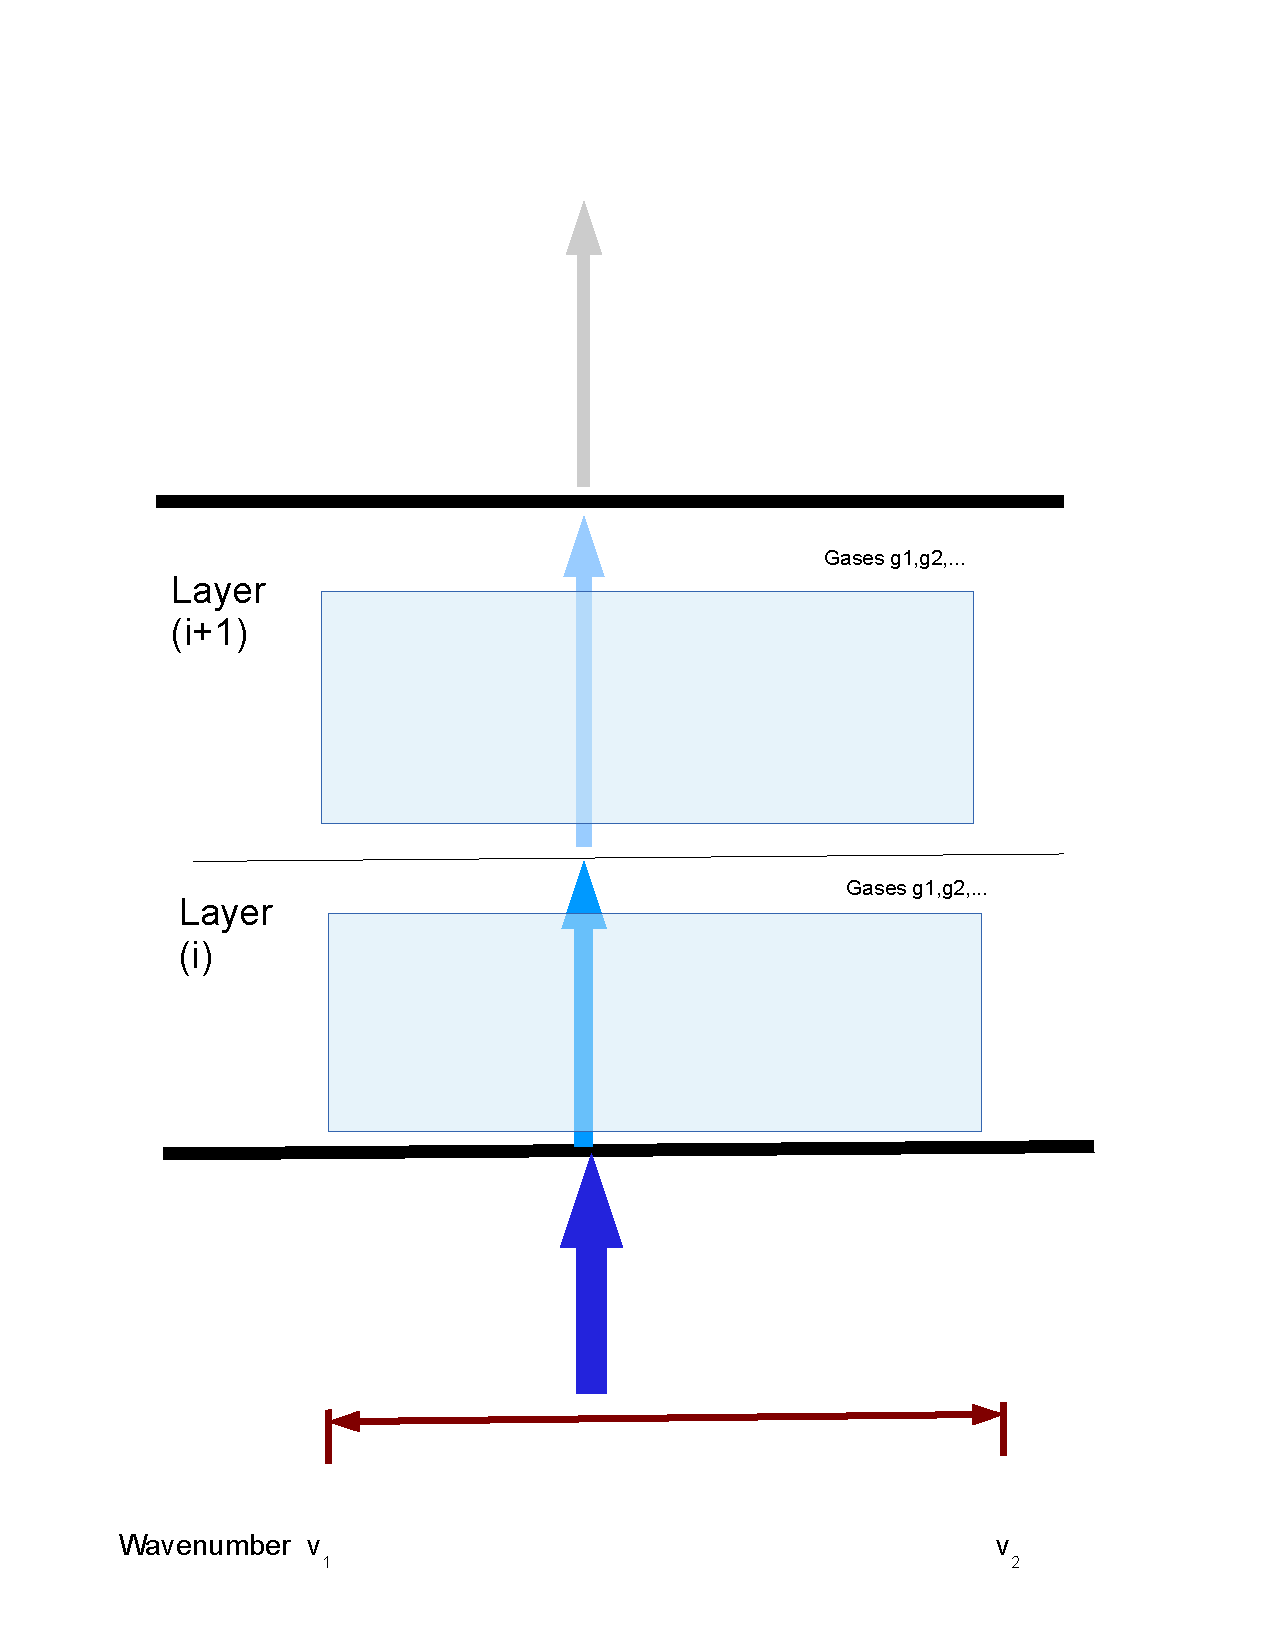
\includegraphics[width=0.45\textwidth]{Figs/twolayers.pdf}
%   \caption{ Pitfalls when applying Beer's law to finite width
%   channels. Not only does it breakdown going from one layer to
%   another, but in addition you cannot simply multiply in the
%   contributions due to different gases }
% \end{wrapfigure}
each layer of the channel in question is parameterized in terms of
predictors such as layer temperature, gas absorber amounts (separated
into water vapor, ozone, other gases) and viewing angle geometry. A
significant complication arises since we are dealing with layer to
space transmittances, coupled with convolutions over finite channel
widths. This leads to a breakdown in Beer's law. In other words, for
example for two consecutive layers, if the monochromatic optical depth
of each is $k(\nu))$ then, the transmittance from the bottom of one
layer to the top of the next, is given monochromatically by
\begin{eqnarray*}
  \tau_{\nu}^{i \rightarrow i+1} & = & \exp(-k_{i}(\nu)) \;\; \exp(-k_{i+1}(\nu)) \\
\end{eqnarray*}
In other words, at each wavenumber, the total transmittance through
both layers, is the product of the transmittances through each layer
\begin{eqnarray*}
  \mathcal{T}(\nu)^{i \rightarrow i+1}           & = &  \mathcal{T}(\nu)^{i} \;\;  \mathcal{T}(\nu)^{i+1}\\
\end{eqnarray*}
where $\mathcal{T}(\nu)^{l}$ is the monochromatic transmittance
through layer $l$.

However, this law breaks down when looking at the convolved
transmittance. For example, for AIRS channel $j$,
\begin{eqnarray*}
  \tau_{\text{AIRS}}^{i \rightarrow i+1}(j) = \int_{\delta \nu_{j}} \exp(-k_{i}(\nu)) \;\; \exp(-k_{i+1}(\nu)) \text{SRF}_{j}(\nu) d\nu
\end{eqnarray*}
which is $NOT$ equal to
\begin{eqnarray*}
  \int_{\delta \nu_{j}} \exp(-k_{i}(\nu)) \text{SRF}_{j}(\nu) d\nu \;\; \int_{\delta \nu_{j}} \exp(-k_{i+1}(\nu)) \text{SRF}_{j}(\nu) d\nu
\end{eqnarray*}
ie
\begin{eqnarray*}
  \mathcal{T}_{\text{AIRS}}^{i \rightarrow i+1}(j) \ne  \mathcal{T}_{\text{AIRS}}^{i}(j) \;\; \mathcal{T}_{\text{AIRS}}^{i+1}(j)
\end{eqnarray*}

The \sa algorithm uses a polychromatic approach by deriving effective
channel-averaged layer-to-space transmittances, which must be done
very carefully since convolved transmittances do not obey Beer's law.
For atmospheric layer $i$, the total monochromatic optical depth is
due to a sum of contributions of all gases $g$ such that
\[
k_i(\nu) = k_i^{g1}(\nu) + k_i^{g2}(\nu) + .... + k_i^{gG}(\nu)
\]
from which the transmittance is $\tau_{i}(\nu) = \Pi_{g=1}^G
\exp(-k_i^{g}(\nu))$. For AIRS channel $j$, the polychromatic
transmittance required for a Fast Model is then
$\mathcal{T}_{\text{AIRS}}^{i}(j) = \int_{\delta \nu_{j}}
\tau_{i}(\nu) d\nu$, and one immediately sees a breakdown of Beer's
law within the individual layers!

% In the making of a Fast Forward Model, monochromatic radiative
% transfer becomes polychromatic radiative transfer, and the above
% needs to be taken into consideration.

The \sa polycrhomatic approach requires special care when there are
different variable gases absorption/emission lines (\ozone, \water,
and \cd) within one \textsf{AIRS} channel. \sa handles this problem by
parameterizing the effective layer-to-space transmittances, and then
converting them to equivalent optical depths for each layer. Further
details are given in \cite{han:02*1,str:02*2}.
\begin{eqnarray*}
  \mathcal{T}^{\text{eff},i}_{\text{AIRS}}(j) & = & \mathcal{T}_{\text{AIRS}}^{i \rightarrow N}(j) / \mathcal{T}_{\text{AIRS}}^{i+1 \rightarrow N}(j) \\
  \mathcal{OD}^{\text{eff},i}_{\text{AIRS}}(j) & = & -ln\{\mathcal{T}^{\text{eff},i}_{\text{AIRS}}(j) \}
\end{eqnarray*}
This means that for each layer $i$ and AIRS channel $j$, we have the
effective optical depth due to all atmospheric gases.
\section{SARTA Cloudy/aerosol sky Radiative transfer algorithm}

Recall from the earlier discussion on monochromatic scattering
radiative transfer, the effects of clouds and aerosols was included by
simply adding in the effective scattering optical depth. For the
polychromatic case, we simply add on the effects of the relevant
scatterer, where needed, and then perform the radiative transfer using
the clear sky algorithm. The only time penalty incurred for each
cloud/aerosol layer, is reading in and interpolating the relevant
scattering tables. Since the scattering parameters vary smoothly in
spectral frequency, it is very straightforward to construct scattering
optical depth tables for the $j$th AIRS channel for scattering species
$S$; then for an arbitrary loading $q(j,i)^{S}$ g/m2
\begin{eqnarray*}
  \text{extinction}(j,i,r)^{S} & = &  \text{extinction}(r)^{S}(1) \times  q(j,i)^{S} \\
  \text{ssa}(j,i,r)^{S} & = &  \text{ssa}(r)^{S} \\
  g(j,i,r)^{S} & = &  g(r)^{S} \\
\end{eqnarray*}
where ssa and $g$ are the single scattering albedo and asymmetry
parameter respectively, and $\text{extinction}(j,r)^{S}(1)$ is the
extinction for a column loading of 1 g/m2; the particle size is
denoted by $r$. The effective optical depths for channel $j$, layer
$i$ are then given by
\[
k_{\text{AIRS,total}}^{j,i} = k_{\text{AIRS}}^{j,i}(\text{gases}) +
\text{extinction}_{\text{AIRS}}^{j,i}(\text{scatterer})
\]
However again, to account for scattering effects, this is
reparameterized as
\[
k\prime_{\text{AIRS}}^{j,i} = k_{\text{AIRS}}^{j,i} \times \{
(1-\omega(j,i) (1-b(j,i)) \}
\]
where the effective single scattering albedo $\omega$ and backscatter
$b$ are obtained from the scatterer-only case $\omega_{0}$ using
\[
\omega(j,i) = \text{ssa}(j,i) \times
\text{extinction}(j,i)/k_{\text{AIRS,total}}^{j,i}
\]
\[
b(j,i) = (1 - g(j,i))/2
\]
after which the radiance at top of the atmosphere can be calculated
using the standard equations of radiative transfer.

\section{Outline for AIRS L2 operational retrievals}

As mentioned earlier, we have already successfully used our code to
retrieve dust loadings and heights, for a sandstorm which eventually
blew over the Mediterranean in late February, 2007 \cite{mac:10}. The
optical depth retrievals agreed with many A-Train sensors, including
MODIS, PARASOL, OMI and Calipso. Out task was arguably made easier by
assuming the dust filled the Field-of-View, fixed particle size
distribution, particle refractive index and effective particle size
(4um diameter). One complication was to also solve for dust height,
instead of using eg climatological heights. For testing purposes, if
the current operational AIRS L1/L2 dust flag detects dust, and we
assume fixed particle sizes and aerosol height from climatology, we
can almost always retrieve dust loadings that correlate very well with
eg MODIS aerosol optical depths, {\em even if they are not necessarily
  accurate because we potentially used an incorrect height}.

We have also prototyped a more complete L2 retrieval in the presence
of dust. Again in this case, we made some assumptions namely we know
the effective particle size and height of the dust, and made a further
assumption that we knew the underlying surface emissivity (over ocean
or land). With these a-priori assumptions, we were able to solve for
$T(z),WV(z)$ and surface temperature, as well as dust loading, using a
1D-var approach.

With the above experience, we outline some suggestions for including
the \sasc code in an operation AIRS L2 retrieval.  The additional
a-priori parameters required would be similar to those we needed for
the dust case, namely cloud fraction, height, particle size and
surface emissivity; in addition we would need cloud phase. Something
similar to the current L2 retrieval could provide estimates of cloud
heights and fractions, from which one could easily produce the
required parameters. This could also be done using atmospheric
profiles (for T(z) and Q(z)) from re-analysis to start.  From the
height(s) one infers phase.  Work is needed to determine if a liquid
cloud particle size must be derived or if climatology can be used.
The re-analysis temperature can be used infer cirrus particle size, or
one can derive it from the observed spectra, especially for the case
of very small cirrus particles which have a very spectrally dependent
emissivity.  This leaves two additional cloud parameters, ice and
water optical depths, although cloud fraction and height will probably
need further adjustment.  One could also think about getting cloud
fraction and height from MODIS.

If dust is detected, which will only happen, in general, when clouds
are minimal, a similar approach can be used to derive the dust optical
depths. 

\section{Implementation details for NWP models}

This section provides some details on converting NWP profiles to a
format that can be used for radiative transfer.  This allows some
testing of both the RTA code and the NWP model clouds.  But, there are
a number of difficulties in this process.  For \sasc we presently only
have two scattering layers implemented.  Thus the NWP profile is
generally turned into a single effective water cloud in one layer, and
a single effective ice cloud, in one layer.  This restriction can be
lifted with some work.  In addition, our algorithm
(\textsf{ecmwf2sarta}) to convert NWP profiles to \sasc input profiles
needs a more sophisticated approach for handling high optical depth
clouds, which should be relatively easy to implement.  The basic
problem at present is that we weight cloud optical depths in all NWP
layers equally, instead of putting higher weights on higher altitude
layers that have sufficient optical depth to render the lower layer
optical depths unimportant in the radiative transfer.

Typically, Numerical Weather Prediction (NWP) models provide
vertically resolved temperature and gas profiles at each grid
point. Both \kc and \sa ingest integrated versions of these profiles
(via the associated \textsf{klayers} code), and use this information
to compute optical depths which are then fed into the radiative
transfer algorithm.

In addition, the NWP models also provide cloud fields at the same
vertical resolution. When developing the \sasc code, we quickly
realized that although liquid water and cirrus profiles were provided,
as were total cloud fractions, we would run into an infinity of
problems implementing cloud fractions, and in particular overlapping
cloud fractions, at each AIRS layer. For this reason, we limit the
\sasc code to having cloud/aerosol in at most \emph{two} slabs. The input
parameters for each of these slabs $k=1,2$ should include
\begin{itemize}
\item species (water cloud, ice (habit) cloud, or aerosol
  (type))
\item particle effective size (in $\mu$m)
\item loading (in g/m2); roughly for ice 50g/m2 = 1 OD, and for water
  2g/m2 = 1 OD
\item cloud/aerosol top (mb)
\item cloud/aerosol bottom (mb)
\item cloud fraction $0 \le c(k) \le 1$
\end{itemize}

In addition, we need a combined cloud fraction $C(k,l)$. For channel
$j$ the total radiance at the top of the atmosphere would then be
\[
R_{\text{AIRS}}(j) = (1 - (c(1) + c(2) - C(1,2)) R_{\text{clear}}(j) +
c(1) R^{(1)}_{\text{cloud}}(j) + c(2) R^{(2)}_{\text{cloud}}(j)
\]
where $R_{\text{clear}}(j)$ is the radiance for a clear column of air,
and $R^{(k)}_{\text{cloud}}$ is the radiance assuming a column of
atmosphere completely filled with cloud of type $k=1,2$. Obviously if
$c(1) = c(2) = C(1,2) = 0$ we get back a clear sky radiance. Depending
on $c(k),k=1,2$ this means at worst, the cloudy sky code is about 3
times slower than the clear sky code.

% One important point is what temperature the cloud is at, if it spans
% pressures (p1,p2) that is thicker than one AIRS layer,
% \textcolor{red}{Need to look at the code!}

\subsection{Types of scatterers}
We currently have scattering tables for a number of species. The
tables span the full range of 2378 AIRS channels and a range of
particle sizes; hence the scattering parameters for an arbitrary
effective particle size is obtained by an interpolation. In addition
the tables are for a particle loading of 1 g/m2; as explained above
the extinction values for an arbitrary loading are obtained by a
simple multiplication.  Possible scatterer types are:
\begin{itemize}
\item aerosol
  \begin{itemize}
  \item desert dust
  \item volcanic ash
  \item effective diameter typically ranges from 0.5 to 10 $\mu$m
  \end{itemize}
\item cirrus cloud
  \begin{itemize}
  \item hex plates
  \item aggregates
  \item effective diameter typically ranges from 10 to 200 $\mu$m
  \end{itemize}
\item water cloud
  \begin{itemize}
  \item effective diameter typically ranges from 15 to 25 $\mu$m
  \end{itemize}
\end{itemize}

\subsection{Cloud levels $\rightarrow$ Slabs}

As mentioned above, we need to go from $\simeq$ 90 levels of cloud
profile information (ECMWF), to two slabs. Our \textsf{ecmwf2sarta}
Matlab routine does the necessary manipulations as summarized below.

\subsubsection{Input requirements}

As stated above, in addition to the usual temperature and trace gas
profiles, we also need the following information from ECMWF/ERA
\begin{itemize}
\item p.ciwc : 91xP cloud ice profiles
\item p.ciwc : 91xP cloud ice profiles
\item p.cc : 91xP cloud total fraction
\end{itemize}

\subsubsection{Smooth the input profiles}
\begin{itemize}
\item Normalize cloud profile eg \\ \hspace{1in}
  $\text{normalized}_{\text{ice}} =
  \text{ice}_{\text{profile}}(:,ii)/\max(\text{ice}_{\text{profile}}(:,ii))$
\item Smooth normalized profile \\ \hspace{1in}
  $\text{normalized}_{\text{ice}} \rightarrow
  \text{normalized}_{\text{ice}}^{\text{smoothed}}$
\end{itemize}

\subsubsection{Turn smoothed profile into slab profiles}
\begin{itemize}
\item Find how many peaks are present in this normalized profile, and
  "width" of peaks.
\item The widths will help determine the cloud top and bottom
\item Start combining peaks so that we have at most two peaks for ice
  cloud, and two peaks for water cloud
\item Finally, combine so at most we have two slabs
\item \emph{This routine needs more work to weight higher optically
    thick clouds more than lower optically thick clouds.}
\end{itemize}

\subsubsection{Determine effective particle sizes, cloud amounts and
  cloud fractions}
\begin{itemize}
\item Cloud amount for each slab is then determined by converting the
  original ice/water cloud profile (in g/g) to integrated g/m2,
\item Effective particle size for water is set to 20 $\mu$m $\pm$ random
  amount
\item Effective particle size for cirrus is set according to the
  temperature of the cloudtop (again, $\pm$ a random amount).
\item Cloud fracs for each cloud, and the overlap, are randomly set
  (using the "cc" field), so that they satisfy
  \begin{itemize}
  \item c(1) $\le$ 1, c(2) $\le$ 1
  \item c(1,2) $\le$ min(c(1),c(2))
  \item clear = 1 - (c(1)+c(2) - c(1,2))
  \item c(1) exclusively = c(1) - c(1,2)
  \item c(2) exclusively = c(2) - c(1,2)
  \end{itemize}
There are more sophisticated overlap schemes that can be used.
\end{itemize}

\subsubsection{Examples}
Figures \ref{fig1}-\ref{fig4} illustrate the results of our
\textsf{ecmwf2sarta} code. Blue and Red are the ECMWF 91 level water
and ice profiles (in g/g) while cyan and magenta are the water and
cirrus output slabs.  The horizontal extent of the slabs are
the integrated cloud profiles, converted to g/m2 and normalized by a
factor of 10000 for the plots. It is possible to modify
\textsf{ecmwf2sarta} code in the future by using a weighting scheme
that uses knowledge of radiative transfer.

\dfigure{Figs/clouds_profile10.eps}{\textsf{ecmwf2sarta} Sample
  1}{fig1}{Figs/clouds_profile100.eps}{\textsf{ecmwf2sarta} Sample
  2}{fig2} \dfigure{Figs/clouds_profile1000.eps}{\textsf{ecmwf2sarta}
  Sample 3}{fig3}{Figs/clouds_profile2000.eps}{\textsf{ecmwf2sarta}
  Sample 4}{fig4}

% \section{Timings}

\section{Comparison to AIRS observations}

We have performed some comparisons of \sasc against AIRS observations.
Figure \ref{AIRS_obs_July} is a gridded map showing daytime AIRS 1231
\wn observations (converted to BT), while Figure \ref{SARTA_calc_July}
is a similar map, showing \sasc calculations, using ERA-Interim
re-analysis fields. Notice the overall similarities in the two
figures. Obvious differences include more/colder deep convective
clouds (DCCs) in the AIRS observations. This map is a combination of
day/night observations as evident by the slope of missing low-latitude
data.  It is interesting to note how well the radiances computed from
ECMWF agree with AIRS observations in the polar regions!
% Since these maps are for July, no daytime AIRS observations are
% possible over the South Polar region.
% \dfigure{Figs/yy_2007_mm_7_airs_global_obs1231_2}{AIRS BT1231 \wn
% observations in July
% 2007}{AIRS_obs_July}{Figs/yy_2007_mm_7_airs_global_eracal1231_2}{\sasc
% calculations for 1231 \wn, using ERA fields for July
% 2007}{SARTA_calc_July}
% Sergio:  need dates for first two figures below.  Also March 11, 2011?
\dfigure{Figs/globalBT1231obs2_crop}{AIRS BT1231 \wn
  observations}{AIRS_obs_July}{Figs/globalBT1231era2_crop}{\sasc
  calculations for 1231 \wn, using ERA fields}{SARTA_calc_July}

The next two figures zoom in on the Pacific/Indian Oceans, for March
10,2011; the \sasc calculations used ECMWF fields, which are higher
resolution in time and space than ERA-Interim.  Figure
\ref{AIRS_obs_March2011} is a gridded map showing daytime AIRS 1231
\wn observations (converted to BT), while Figure
\ref{SARTA_calc_March2011} is a similar map, showing \sasc
calculations. Althought there are many general similarities, the cloud
fields are quantitatively quite different.  In general the ECMWF
computed clouds are spread wider spatially.  

\dfigure{Figs/airs_bt_image}{AIRS BT1231 \wn observations for March
  11, 2011}{AIRS_obs_March2011}{Figs/ecmwf_bt_image}{\sasc
  calculations for 1231 \wn, using ECMWF fields for March 11,
  2011}{SARTA_calc_March2011}

\section{Comparison to Other RTA Algorithms}

We have done some limited comparisons of \sasc against \pcrtm,
which is a fast radiative transfer code trained using DISORT, that
uses principal components for the radiative transfer.  Note
that in the discussion in this section is very different from Section
5, where we outlined a plan for an AIRS L2 retrieval algorithm.

The \pcrtm implementation we compare against uses 50 random subcolumn
incarnations of maximal overlap clouds. Since it is impossible for a
finite resolution NWP grid to resolve the fine structure of clouds, an
improvement on the simulation of radiances would include an average of
several instances of clouds built from the NWP fields (ie use sub-grid
points). In particular, the overlapping and extent of the clouds at
different subgrid points can also be varied, ranging from all at fixed
locations, to clouds at various locations within the subgrid.  Other
differences are that the \pcrtm implementation uses ice cloud sizes
that vary between 50 to 125 um, fixed 20 um water sizes, and Ping
Yang's scattering parameters.

For all discussions in this section, ECMWF profiles were used in running
both \sasc and \pcrtm.

\dfigure{Figs/spectra_sartaVSpcrtm.jpg}{Comparing \sasc vs
  \pcrtm}{spectra}{Figs/pcrtm_calc_vs_sarta_biasV1}{BT1231
  comparisons}{bt1231_sarta_pcrtm}

Figure \ref{spectra} is a 2d histogram, showing bias between the two
codes as a function of wavenumber. The thick black line is the mean of
the bias, while the blue lines are one standard deviation away; the
colorscale is the log of the number of instances. The figure shows
that typically \sasc produces brightness temperatures that are about 3
$\pm$ 4 K warmer than \pcrtm, for window channels. This could arise
from a number of factors, such as too few cirrus cloud (either
amount or fraction). More likely, though, is our use of such a simple
scheme to map NWP clouds to two scattering layers.  This too simple
approach will center the cloud around the peak, or centroid, of the
cloud optical depth, producing significantly warmer emission
temperatures for thick clouds where one only observes the cloud-top
temperature. However, this use of 50 statistical variations in cloud
overlap may also be the cause of difference between \sasc and \pcrtm.
\emph{For L2 retrievals, these differences will become largely
  unimportant since only 1-2 cloud layers can be retrieved in any case.}

% Sergio, I don't see this at all?  Labels for too small in this
% figure.
% To alleviate this, it is possible to tweak our
% \textsf{emcwf2sarta} code, as mentioned in section 4.2.5. Figure
% \ref{bt1231_sarta_pcrtm} shows the BT1231 \wn bias between \pcrtm and
% \sasc, as a function of computed \pcrtm temperature. The colorscale is
% the log of the number of observations, and shows that the differences
% typically begin to manifest at about 260 K.

% \dfigure{Figs/pcrtm_vs_sarta_vs_obs_pdf1231_allregions_2.jpg}{Comparing
%   \sasc vs \pcrtm vs AIRS observations, over all the
%   globe}{pdf_airs_sarta_pcrtm}{Figs/pcrtm_vs_sarta_vs_obs_pdf1231_pacific_2.jpg}{Comparing
%   \sasc vs \pcrtm vs AIRS observations, over the Tropical
%   Pacific}{pdf_airs_sarta_pcrtm_tropical_pacific}.

% Figures \ref{pdf_airs_sarta_pcrtm} and
% \ref{pdf_airs_sarta_pcrtm_tropical_pacific} shows the BT1231 \wn pdfs
% over all points on the globe, and over the Tropical Pacific. In each
% case, blue, red and black are the \pcrtm, \sasc and AIRS observations,
% respectively. As expected from the above discussion, typically \sasc
% is "warmer" than \pcrtm, but it is not easy to chose between the two
% when comparing to the AIRS observations.


% Sergio:  you have *got* to make the sign clear in any figures 
% showing a difference!!  Like the two figures below!!  What is being
% subtacted from what!  It should *not* just be in the title, which
% people often don't look at.  It should be in the caption!  In fact,
% figures in papers should not have titles!
While the speeds of the two codes are very similar, the architecture
of our \sasc is very much the same as the clear sky \sa code, and so
should be easy for a new user to learn. Figures \ref{pdf1_sarta_pcrtm}
and \ref{pdf2_sarta_pcrtm} shows the night time biases between \sasc
and \pcrtm for 820, 960, 1231 and 2616 \wn over all points on the
globe (SARTA minus PCRTM). The graph on the left uses the 50 subcolumn
version of \pcrtm while the one on the right shows a one subcolum
version.  This suggests that the NWO overlap statistics significantly
affect the output of PCRTM, making the radiances colder.  Figure
\ref{pdf2_sarta_pcrtm} shows better agreement, and the remaining
differences are likely to do our too-simple NWP cloud optical depth
weighting scheme.

\dfigure{Figs/pcrtm_calc_vs_sarta_calc_histV1.jpg}{Comparing \sasc vs
  \pcrtm (50
  subcolumns)}{pdf1_sarta_pcrtm}{Figs/pcrtm_calc_vs_sarta_calc_histV2.jpg}{Comparing
  \sasc vs \pcrtm (1 subcolumn)}{pdf2_sarta_pcrtm}

% Importantly, even though there is a bias between the \sasc and \pcrtm
% calculations, this should not impact an operational temperature and
% humidity retrieval. An operational infrared AIRS L2 retrieval would
% need to \emph{accurately account} for scattering effects when solving
% for temperatures and humidity. Clearly using NWP model fields which
% have tremendous variability, our code is producing radiances that
% match those from \pcrtm. So it should be very possible improve the
% AIRS L2 retrievals in the presence of clouds (and aerosols) using
% \sasc. This is different from a requirement to accurately solve for
% cloud heights, phases, particle sizes and loadings, which was noted in
% the first paragraph of Section 5, where we pointed out we could always
% retrieve a dust loading, even though it was not necessarily correct
% because we potentially used an incorrect height.

\bibliographystyle{unsrt}
% \bibliography{/home/sergio/PAPERS/BIB/atmspec2002}
\bibliography{/Users/strow/Tex/Bib/atmspec2002}

\end{document}
